\section{Experimental Setup}
\label{exp}

To evaluate the performance of Viscous, we compare the Viscous with popular transport protocols MPTCP, MPQUIC\cite{mpquic-measure}, TCP and QUIC with different network configurations. We performs three different experiments, a) general evaluation with rocket fuel topology, b) aggregated benefit measurement and c) mobility analysis. The Mininet platform is used to perform experiments on rocket fuel topology and aggregated benefit measurement and Raspberry pi board is used to perform experiments on mobility analysis. 

The mininet provides capability of generating different type of network topology with different network conditions in a single system and run any existing real network application on the Mininet generated network. Raspberry pi board setup give us capability to create physical network and run applications on low end devices.

For the Mininet based experiments, we use a computer with 8GB RAM, 4 core GenuineIntel i5-4590 CPU with 3.30 GHz clock frequency. It is equipped with Ubuntu 16.04.1 operating system with Linux kernel version 4.4.70 with the MPTCP v0.92 and the Mininet 2.2.2. For the Rapsberry pi setup, we use Raspberry Pi model 3.
To compare with the QUIC and the MP-QUIC, we use golang implementation of the MP-QUIC by Conick {\it et. al.}~\cite{mpquic-measure} which is a extension of \texttt{golang} implementation of the QUIC~\cite{quic-go}.

\subsection{Setup for General Evaluation with Rocketfuel Topology}
\label{expsetup-rocketfuel}
The RocketFuel topology is a standard topology generated by using {\tt traceroute} from different locations all over the globe to different servers \cite{Spring:2004:MIT:973492.973494}. We take a topology with 29 different networks connected via 15 routers. We place 14 host inside different networks. Among these 14 hosts, we connect 7 hosts with two different networks (we call it client host) and other 7 hosts with a single network (server host). So, there are 7 pair of server-client host. In this topology we use 3 different bandwidth for different links i.e. core link, server link, and client link. A core links connects a switch with a router with 100mbps bandwidth and 3ms delay, a server link connects a server and a switch with 50mbps bandwidth and 2ms delay. We keep 10mbps bandwidth for client link connecting a client host and a switch while varying the delay over different experiment.

In experiments, we sent data from each server host to their dedicated client host using different protocols (Viscous, QUIC, MPQUIC, TCP and MPTCP) and other way around. We call forward experiment when we send traffic from server host to client host and reverse experiment when we send data from client host to server host.

In this experiment, we vary client link delay and number of simultaneous thread. Then we send $50$\footnote{Golang implementation of QUIC and MP-QUIC does not support more than $50$ connections.} back-to-back connection through each thread with payload varied using exponential distribution with mean $25$ KB\footnote{We decided $25$ KB as our initial observation with multiple rich webpages (web page with lots of images and embedding) yields mean HTTP response size of $~25$ KB.}. 

\subsection{Setup for Aggregated Benefit Measurement}
To compare Viscous with other protocol in various network conditions, we perform similar experiment performed by \cite{mpquic-measure,Paasch:mptcp:compare}. We perform these experiments with various of scenarios by changing basic network parameters {\it e.g.} link bandwidth, RTT, queuing delay and packet loss rate. These experiments are performed using simple topology shown in Fig.~\ref{fig:aggregation_dia} with the help of Mininet network emulator. We run experiments on approximately 150 scenarios generated using WSP space filling algorithm described in \cite{wspalgo} from configuration space described in Table~\ref{tbl:noloss_param}. Three experiments are performed on each scenario for each protocol. We run experiments on TCP and QUIC for both the paths and compared with best performance. We also observed that the MPTCP depends on initial path selection, so we run experiments with MPTCP for both the paths and compared with best and worst initial path performance. We considered Goodput as the metric of performance. In each of these experiments, we send 50 back-to-back request-response over a single thread. The client request for a payload size (in number of bytes) to server and the server transfer the requested amount of payload to client. We vary response size with a exponential distribution with mean $25$ KB payload.
\begin{equation} \label{eqn:agre_benefit}
Ben(S) = 
\begin{cases}
\frac{G_v - G_p^{max}}{G_v - G_v^{max}} & \text{if } G_v > G_V^{max} \\
\frac{G_v - G_p^{max}}{G_v^{max}} & \text{otherwise}
\end{cases}
\end{equation}

To measure aggregative benefit, we followed modified equation provided in \cite{Kaspar:2012:MAH:2206765.2206770,Paasch:mptcp:compare,mpquic-measure}
as Equation~(\ref{eqn:agre_benefit}). Here we measure the benefit of using Viscous instead of other protocol for a given scenario $S$. Here $G_v$ is the mean Goodput found in all experiments using Viscous for the scenario $S$, $G_p^{max}$ is the max of mean Goodput found in each path for single path protocol while $G_p^{max}$ is mean Goodput achieved by a multi-path protocol. The value of $Ben(S)$ is in between -1 to 1, while -1 mean Goodput of other protocol is twice good as Viscous while 1 mean, Goodput of other protocol is 0, and if $Ben(S)$ is 0, other protocol perform exactly same as Viscous.

\begin{figure}
	\centering
	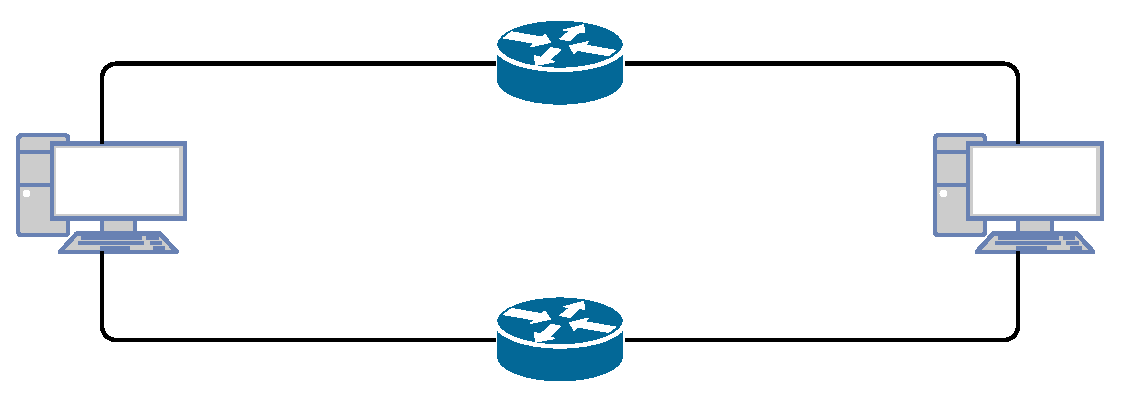
\includegraphics[width=\linewidth]{img/aggregation.eps}
	\caption{\label{fig:aggregation_dia}Network used to find aggregative benefit}
\end{figure}

\begin{table}[h]
	\centering
	\begin{tabular}{l||c|c||c|c}
		%		\hline
		& \multicolumn{2}{c||}{Low-BDP} & \multicolumn{2}{c}{High-BDP}\\
		\hline
		\hline
		Capacity [Mbps] & 0.1 & 100 & 0.1 & 100 \\
		\hline
		Propagation delay [ms] & 0 & 50 & 0 & 400 \\
		\hline
		Queuing [ms] & 0 & 100 & 0 & 2000 \\
		\hline
		Loss rate [\%] & 0 & 2.5 & 0 & 2.5 \\
		%		\hline
	\end{tabular}
	\caption{\label{tbl:noloss_param}Scenario used}
\end{table}

\subsection{Setup for Mobility Analysis}
We perform an experiment on mobility. To test this feature, we prepare the test platform using Raspberry Pi 3. We have depicted the setup diagram in Fig.~\ref{fig:mobility_diagram}. There are total five Raspberry pi acting as routers, this are R1, R2, R3, R4 and RW1. Two host T1 and T2 with this setup. The T1 host directly connected to R1. The host T2 connected to RW1 using WiFi channel. The T2 host is also connected to R3, R4 router via wire. The host T2 can stay connected with R4 or R3 at a time, not with both. All the links except link between RW1 and T2 in this setup are wired link.

To performs the experiment, we start sending data from T2 to T1 while T2 is connected with R4 via wired link and RW1 via WiFi. While the Viscous connection is live, we disconnect T2 from R4. After few seconds, we connect T2 with R3. 
\begin{figure}
	\centering
	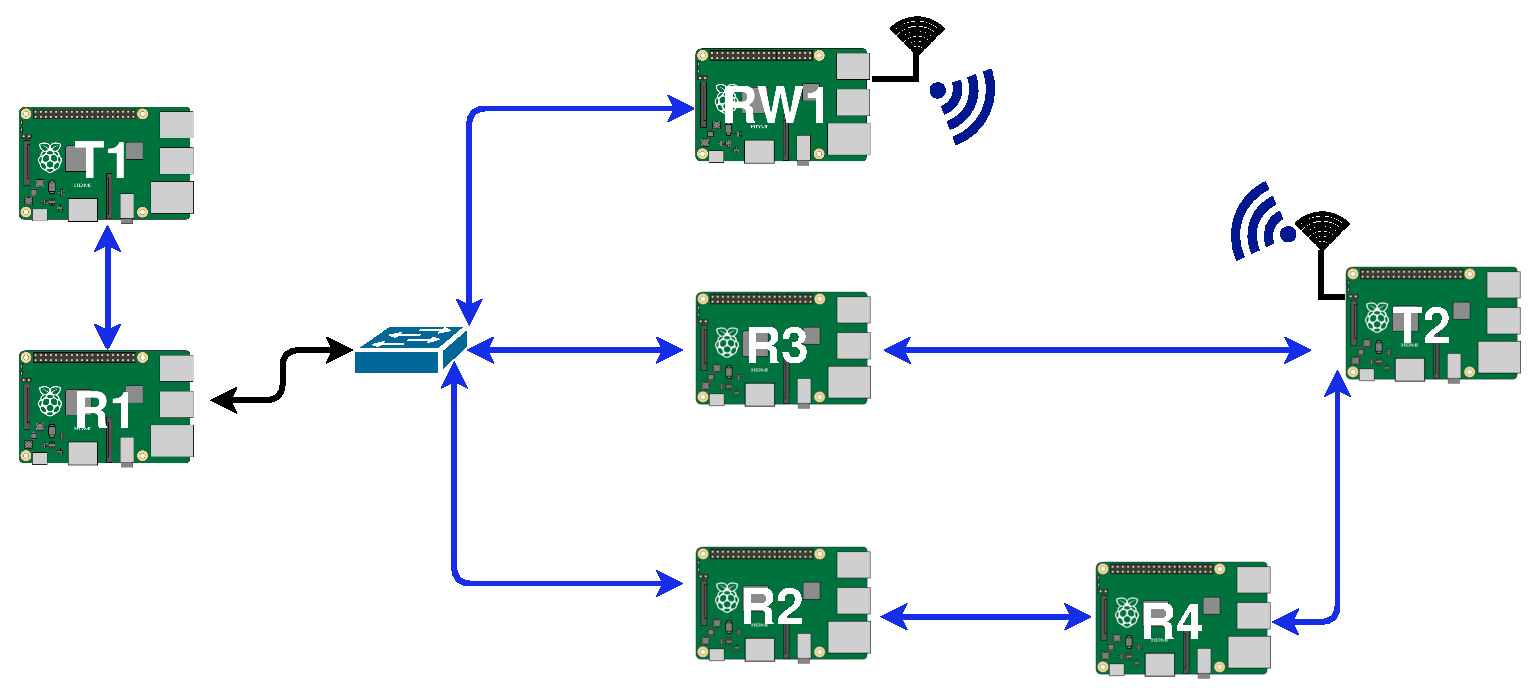
\includegraphics[width=.9\linewidth]{img/mobility/demo-Diagram.eps}
	\caption{\label{fig:mobility_diagram}Raspberry pi setup to test the mobility of viscous}
\end{figure}

